%----------------------------------------------------------------------------------------
%	PACKAGES AND OTHER DOCUMENT CONFIGURATIONS
%----------------------------------------------------------------------------------------

\documentclass[
11pt, % The default document font size, options: 10pt, 11pt, 12pt
english, % ngerman for German
singlespacing, % Single line spacing, alternatives: onehalfspacing or doublespacing
headsepline, % Uncomment to get a line under the header
]{MastersDoctoralThesis} % The class file specifying the document structure
\usepackage[utf8]{inputenc}
\usepackage{float}
\usepackage{subcaption}
\usepackage{amssymb}
\usepackage{graphicx}
\graphicspath{ {images/} }
\usepackage{amsmath}
\usepackage[T1]{fontenc} % Output font encoding for international characters
\usepackage{mathpazo} % Use the Palatino font by default
\usepackage[backend=bibtex,style=authoryear,natbib=true]{biblatex} % Use the bibtex backend with the authoryear citation style (which resembles APA)
\addbibresource{example.bib} % The filename of the bibliography
\usepackage[autostyle=true]{csquotes} % Required to generate language-dependent quotes in the bibliography

%----------------------------------------------------------------------------------------
%	MARGIN SETTINGS
%----------------------------------------------------------------------------------------

\geometry{
	paper=a4paper, % Change to letterpaper for US letter
	inner=2.5cm, % Inner margin
	outer=3.8cm, % Outer margin
	bindingoffset=.5cm, % Binding offset
	top=1.5cm, % Top margin
	bottom=1.5cm, % Bottom margin
	%showframe, % Uncomment to show how the type block is set on the page
}

%----------------------------------------------------------------------------------------
%	Document INFORMATION
%----------------------------------------------------------------------------------------

\thesistitle{Design and Implementation of a software package for Engineering drawing} % Your thesis title, this is used in the title and abstract, print it elsewhere with \ttitle
\supervisor{Dr. Subashish \textsc{Banerjee}} % Your supervisor's name, this is used in the title page, print it elsewhere with \supname
\examiner{} % Your examiner's name, this is not currently used anywhere in the template, print it elsewhere with \examname
\degree{Bachelor of Technology} % Your degree name, this is used in the title page and abstract, print it elsewhere with \degreename
\author{Shreshth \textsc{Tuli}} % Your name, this is used in the title page and abstract, print it elsewhere with \authorname
\addresses{} % Your address, this is not currently used anywhere in the template, print it elsewhere with \addressname

\subject{Biological Sciences} % Your subject area, this is not currently used anywhere in the template, print it elsewhere with \subjectname
\keywords{} % Keywords for your thesis, this is not currently used anywhere in the template, print it elsewhere with \keywordnames
\university{\href{http://www.university.com}{Indian Institute of Technology, Delhi}} % Your university's name and URL, this is used in the title page and abstract, print it elsewhere with \univname
\department{\href{http://www.cse.iitd.ernet.in/}{Department of Computer Science and Engineering}} % Your department's name and URL, this is used in the title page and abstract, print it elsewhere with \deptname
\group{COP290} % Your research group's name and URL, this is used in the title page, print it elsewhere with \groupname
\faculty{\href{http://faculty.university.com}{Faculty Name}} % Your faculty's name and URL, this is used in the title page and abstract, print it elsewhere with \facname

\AtBeginDocument{
\hypersetup{pdftitle=\ttitle} % Set the PDF's title to your title
\hypersetup{pdfauthor=\authorname} % Set the PDF's author to your name
\hypersetup{pdfkeywords=\keywordnames} % Set the PDF's keywords to your keywords
}

\begin{document}

\frontmatter % Use roman page numbering style (i, ii, iii, iv...) for the pre-content pages

\pagestyle{plain} % Default to the plain heading style until the thesis style is called for the body content

%----------------------------------------------------------------------------------------
%	TITLE PAGE
%----------------------------------------------------------------------------------------

\begin{titlepage}
\begin{center}

\vspace*{.06\textheight}
{\scshape\LARGE \univname\par}\vspace{1.5cm} % University name
\textsc{\Large Mathematical Model}\\[0.5cm] % Thesis type

\HRule \\[0.4cm] % Horizontal line
{\huge \bfseries \ttitle\par}\vspace{0.4cm} % Thesis title
\HRule \\[1.5cm] % Horizontal line
 
\begin{minipage}[t]{0.4\textwidth}
\begin{flushleft} \large
\emph{Authors:}\\
\authorname\\
Sankalan Pal \textsc{Chowdhury}
\end{flushleft}
\end{minipage}
\begin{minipage}[t]{0.4\textwidth}
\begin{flushright} \large
\emph{Supervisor:} \\
\href{http://www.cse.iitd.ernet.in/~suban/}{\supname} % Supervisor name - remove the \href bracket to remove the link  
\end{flushright}
\end{minipage}\\[3cm]
 

\includegraphics[width=100pt]{logo} \\
\vfill
Course: Design Practices - \groupname\\\deptname\\[2cm] % Research group name and department name
Developed on \LaTeX
 
\vfill

{\large January 18, 2018}\\[4cm] % Date
%\includegraphics{Logo} % University/department logo - uncomment to place it
 
\vfill
\end{center}
\end{titlepage}


%----------------------------------------------------------------------------------------
%	THESIS CONTENT - CHAPTERS
%----------------------------------------------------------------------------------------

\mainmatter % Begin numeric (1,2,3...) page numbering

\pagestyle{thesis} % Return the page headers back to the "thesis" style

\chapter{3D Transformations}
Once a 3D object has been built, we need to be able to transform it in various ways. Below, we describe three families of such transforms
\section{Translation of 3D Object}
Translation is perhaps one of the most basic operations that can be performed on an object. It can be defined simply as the elementary transform which can preserve relative positions of any two points in space.
Mathematically, it is defined as:\\
\begin{align*}
T_{x_0y_0z_0}((x, y, z)) = ((x + x_0, y + y_0, z + z_0))
\end{align*}
While this is almost trivial to implement, we would still resort to libraries for the sake of continuity.

\section{Scaling of 3D Object}
Scaling is a linear transformation that enlarges or shrinks an object by scale factors that may or may not be equal in all directions. The scaling matrix is any diagonal matrix with positive reals as elements. Should the scaling be uniform, the scaling matrix takes the special form kI where $k\,\epsilon   \,{\rm I\!R}^+$ is the scaling factor and I is the $3^{rd}$ order Identity matrix.\\
While scaling is definitely an important type of transform, It is not generally used in Engineering Drawing.

\section{Rotation of a 3D Object}
Rotation in 3D may be imagined in multiple intuitive ways. However, for mathematical treatment, it is necessary to formulate rotation formally. Hence, we define rotation as any linear function from ${\rm I\!R}^3$ to $ {\rm I\!R}^3$ that has the following properties:
\begin{itemize}
  \item There exists a line in the space that is same as its image. This line is called the Axis of Rotation(AoS). For simplicity, we assume that $(0,0,0)^T$ lies on this axis.
  \item The distance between any two points is same as the distance between their images.
\end{itemize}

\section{Matrix Representation}
Since our function is a linear map from ${\rm I\!R}^3$ to ${\rm I\!R}^3$, it can be represented in the form of a 3x3 Matrix. We begin with the most general form of this matrix:
\begin{align*}
\begin{bmatrix} 
a_{11} & a_{12} & a_{13} \\
a_{21} & a_{22} & a_{23} \\
a_{31} & a_{32} & a_{33} \\
\end{bmatrix}
\end{align*}
This has a total of 9 degrees of freedom. Hereon, we try to discover constraints that can reduce this.

\section{Preservation of Distances}
Since rotations preserve distances, between any two arbitrarily chosen points it must also preserve distance between $(0,0,0)^T$  and $(1,0,0)^T$. Now the image of $(0,0,0)^T$ is $(0,0,0)^T$  whereas the image of $(1,0,0)^T$ is $(a_{11}, a_{21}, a_{31})^T$ , so we must have 
\begin{align*}
a_{11}^2+a_{21}^2+a_{31}^2=1
\end{align*}
This same technique can be applied to $(0,1,0)^T$ and $(0,0,1)^T$ to obtain the relations:
\begin{align*} a_{12}^2+a_{22}^2+a_{32}^2=1 \\ a_{13}^2+a_{23}^2+a_{33}^2=1 \end{align*}
These equations show that in each column, only two parameters are independent. \\
Now, consider the three points $O(0,0,0)^T$, $B(1,0,0)^T$  and $C(0,1,0)^T$. Since rotation would preserve pairwise distances, the triangle formed by their images $(O’B’C’)$ would be congruent to the triangle $OBC$. Since we know that $O’ = O$, 
\begin{align*} \angle B'OC'= \angle BOC = 90^{\circ} \end{align*}
Which implies that the dot product between B’ and C’ must be zero. This implies that
\begin{align*} a_{11} a_{21}+a_{12} a_{22}+a_{13} a{_23}=0\end{align*}
Similar manipulations with other points can show that any pair of columns are orthogonal. These, and the previous relations can all be captured in the following constraint:
\begin{align*} \sum_{j=1}^3 a_{ij}a_{kj} = \delta_{ik} \end{align*}
Where $\delta_{ik}$ is the Kronecker delta. Two implications follow:
\begin{itemize}
  \item The matrix under question is Orthogonal, i.e. its transpose is same as its inverse
  \item Since there are 6 constraints on 9 variables, only three of these variables can be independent
\end{itemize}
Till now we have only used the fact that the Origin is invariant under rotation. The fact that the entire axis remains invariant actually adds the further constraint that the determinant of the Matrix is +1 ( and not -1 ). \\
Specifying an arbitrary axis passing through the origin takes two parameters. To define a rotation completely, we must have one more parameter. This is taken to be the Angle of rotation.\\ \\
\emph{Definition:}\\
Let $P$ be a point not lying on the Axis of rotation. Let $P’$ be its image and $P"$ be its projection onto the AoS.  $\angle PP"P’$ can be proven to be independent of the choice of $P$ and is known as the axis of rotation.

\section{Simpler Cases}
The 2D version of the rotation problem is rather easy to calculate. A 2D rotation by an angle $\theta$ about the origin is characterized by the matrix:
\begin{align*}
\begin{bmatrix} 
cos\theta & -sin\theta \\
sin\theta & cos\theta\\
\end{bmatrix}
\end{align*}
The derivation is rather easy and can be inferred from the following figure:\\
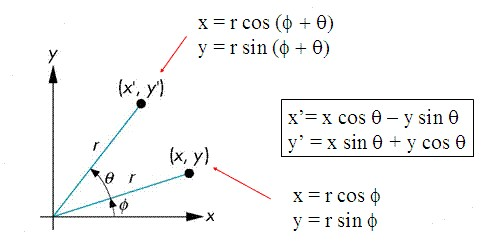
\includegraphics{img1}
Now, rotation in 3D about $Z$ axis by angle $\theta$ can be seen as simply transforming the $X$ and $Y$ coordinates using the above matrix and keeping the $Z$ coordinate unchanged. This gives us the matrix:
\begin{align*}
M_Z(\theta) = 
\begin{bmatrix} 
cos\theta & -sin\theta & 0 \\
sin\theta & cos\theta & 0\\
0 & 0 & 1 \\
\end{bmatrix}
\end{align*}
But there is nothing special about the the $Z$ axis, and we can similarly obtain rotation matrix for rotation about $X$ and $Y$ Axes in the same way.\\
\begin{align*}
M_X(\theta) = 
\begin{bmatrix} 
1 & 0 & 0 \\
0 & cos\theta & -sin\theta \\
0 & sin\theta & cos\theta \\
\end{bmatrix} \\
M_Y(\theta) = 
\begin{bmatrix} 
cos\theta & 0 & sin\theta \\
0 & 1 & 0 \\
-sin\theta & 0 & cos\theta \\
\end{bmatrix}
\end{align*}

\section{Putting it together}
We now construct the general 3D rotation matrix.\\
Let the axis of rotation be define parametrically as $ (r\, sin \alpha \, cos \beta, r\, sin \alpha \,sin \beta, r \, cos\alpha ) $ with r as a parameter. Also, let $\theta$ be the Angle of rotation. We seek to find out $M(\alpha, \beta, \theta )$. \\ \\
Had our axis coincided with the Z axis, we would have $M (0,0,\theta ) = M_Z(\theta)$. However, when that is not the case, we can still use this if we can perform suitable rotations to bring the Axis of Rotation to $Z$ axis. \\ \\
Once the rotation has been performed, our rotations can be reversed, and the Axis of rotation brought to its original rotation. This involves 5 steps:
\begin{enumerate}
\item Rotate around $Z$ axis by angle $\beta$ to bring AoS to the $XZ$-Plane.
\item Rotate around $Y$ by angle $\alpha$ to make AoS coincide with $Z$ axis.
\item Rotate around $Z$ axis by $\theta$.
\item Invert step 2.
\item Invert step 1.
\end{enumerate}
All in all, we get: \\
\begin{align*}
M(\alpha, \beta, \theta) = M_Z^T(\beta) \, M_Y^T(\alpha) \, M_Z(\theta) \, M_Y(\alpha) \, M_Z(\beta)
\end{align*}
At this point, Simplification becomes a mere computational task. For our purpose, we would leave this up to standard Libraries.






\chapter{3D - 2D Conversion}
A basic purpose of the tool we are working on would be to generate a 3D model from a given set of orthographic projections. Further, we should also be able to generate all possible projections given a 3D model. In this aspect, being able to Convert between 2D and 3D becomes essential.\\ \\
\emph{Note: In the rest of the document it is assumed that objects do not consist of curved edges or surfaces}
\section{Representation}
2D projections are normally presented in Engineering drawing as a labelled wire-frame with separate patterns for visible(solid) and hidden(dashed) lines. To represent this in our program, we shall use a Eulerian graph with labeled vertices and separate sets of visible and hidden edges.\\
 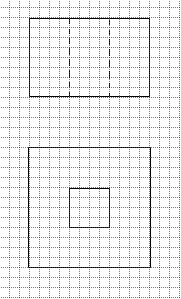
\includegraphics[height = 250pt]{2d-3d-1}
\hspace{42mm} 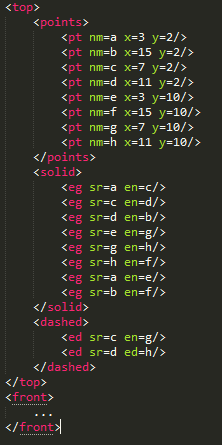
\includegraphics[height = 250pt]{2d-3d-2} \\
(description shown here is not final, and may change subject to programming requirements)\\ \\
The 3D representation is much more internal, and would be visible to the user only through projections. We propose to use a similar description, except for having faces enumerated as well. This would become important for separating solid edges from dashed ones.

\section{Projection: From 3D to 2D}
We have already discussed at length how points can be rotated and transformed in 3D space. Since edges and planes are attached to points that surround them, they also get rotated along with points. To project a certain orthographic view, we shall use the following technique:
\begin{enumerate}
\item Rotate the object so that the plane of interest coincides with the XY plane.
\item Start off from the point having Z coordinate farthest from the viewer. 
\item Drop the Z coordinate to project points onto the drawing plane. Do this in the order that points farther from the viewer get projected first.
\item Whenever both end points of an edge have been projected, create the edge as solid.
\item Whenever all bounding points of a plane have been projected, calculate the region covered by the plane. Change any solid lines in this region to dashed lined.
\item Finish when all points have been projected.
\end{enumerate}
A good implementation of this routine should be able to run in $O(F+E+V)$. Using Euler’s Characteristic formula, this is same as $ O(V)$ where $V$ is the number of vertices.
Note that at this point, we have not lost invertibility. We can show this using the example considered above.





\section{Reconstructing: From 2D to 3D}

Here, we consider the problem of generating a 3D wireframe given an orthographic projection (front and top) that was generated from a wireframe using the above algorithm at the first place.\\ \\
\begin{center}
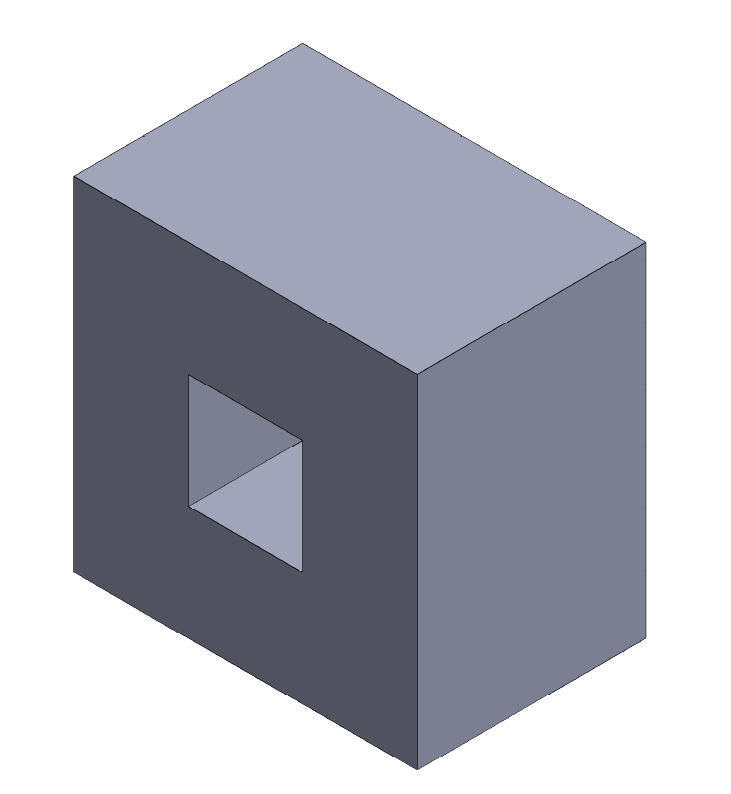
\includegraphics[width = 200pt]{solid} \\
\emph{Exemplar 3D Solid object}
\end{center}

\subsection{Modeling though example}

\begin{center}
    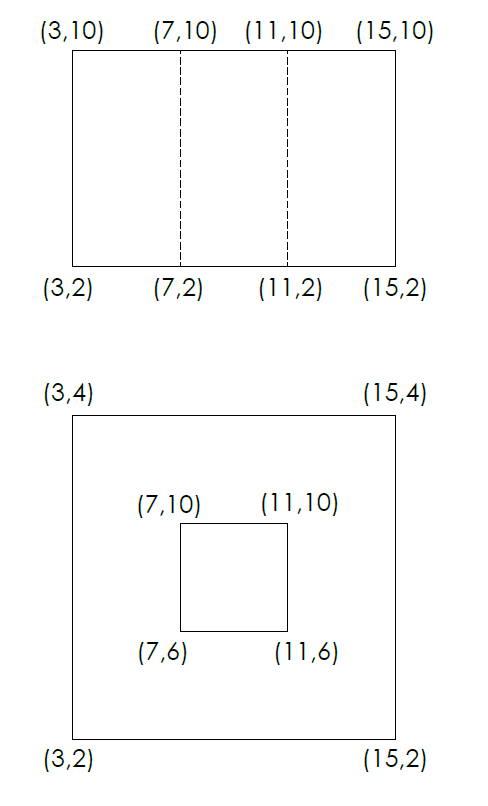
\includegraphics[width=0.5\textwidth]{ortho}\\
    \emph{Otho graphic view}
\end{center}
The input here consists of a pair of vectors of tuples giving the projected points in top and front views. The edge sets would be identical, except some solid edges becoming hidden and vice versa. The most important fact here is that there must be a one-to one correspondence between vertices in both (or all three) of the views.\\ \\
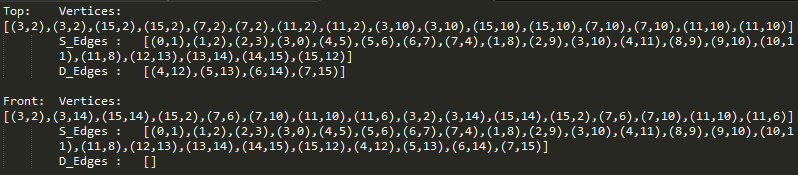
\includegraphics[width=\textwidth]{2d-3d-3}\\ \\
Note that the order of vertices is actually defining a labeling for them, and is therefore fixed. The order of edges is, however, variable.\\ \\
Should we have this kind of an input, we can easily create a deterministic algorithm. \\ \\
Let $(X_{ti}, Y_{ti})$ be the $i^{th}$ vertex in the top view, $(X_{fi}, Y_{fi})$ be the $i^{th}$ vertex in the front view, and $N_t, N_V$ be the cardinality of these sets respectively.

Further, let $S_t\, H_t \subset \{ (a,b) \, | \, a,b \subset (0,1,2,... N_t), a \neq b \} $ be the set of Solid and Hidden edges for the top view and, $S_f\, H_f \subset \{ (a,b) \, | \, a,b \subset (0,1,2,... N_f), a \neq b \} $ be that for the front view. \\ \\
The given set of inputs is a valid orthographic projection if:
\begin{enumerate}
\item $N_t = N_V$ 
\item $x_{ti} = x_{fi}$ for all valid i
\item $S_t \cup H_t = S_f \cup H_f$
\end{enumerate}
The original members vertex set $V(x_i, y_i, z_i)$ can then be represented as: $x_i = y_{ti}$, $y_i = -y_{fi}$, $z_i = -x_{ti}$. This would be correct except the possibility of a translation to the entire object, and fully correct when seen in relative terms.\\ \\
The edge set is even easier to recover. We simply have $E = S_t \cup H_t$. \\ \\
Recovering the set of faces is more complex though. In principle, every cycle in the graph may represent a face. This is in fact a good place to begin. Thereafter, we need to apply the following two filters:
The given set of inputs is a valid orthographic projection if:
\begin{enumerate}
\item If one face completely contains another face, then the second face must actually be a hole in the first.
\item No three faces can share the same edge as boundary. If they do, nne of the faces must be falsely identified. 
\end{enumerate}
This kind of an input, though easy to invert, is hardly ever available from a user. The closest one can get then, is when all vertices of the drawing are labeled. Even then, more often than not, there can be a discrepancy w.r.t. which edges exist and which do not.

\subsection{Implementation of example}
We try to apply this procedure to the example considered above. First comes the part of Recovering vertices. In O(V) time, a rather naive algorithm can return:\\ \\
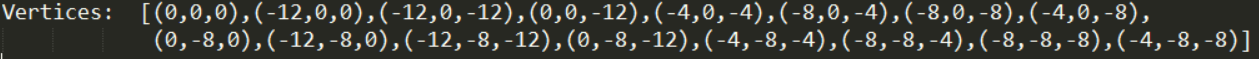
\includegraphics[width=\textwidth]{2d-3d-6}\\ \\
Note that apart from matching, the origin has also been shifted to the first point. This choice is arbitrary, but, nevertheless, logical. The edges are essentially just copied. \\ \\
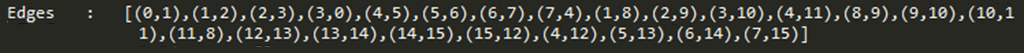
\includegraphics[width=\textwidth]{2d-3d-7}\\ \\
Next comes the faces. An algorithm for discovering all cycles in a graph is not too hard, and there exists efficient algorithms like Johnson’s Algorithm to do this in less than quadratic time. We, however, need not use such an implementation, as not all cycles are of interest to us. In fact, we are only looking at cycles which have all points lying on the same plane. But first, we state an obvious theorem.\\ \\
\begin{center}
\emph{From every vertex defined in a polyhedron, there must exist three or more edges originating from it of which no three can be coplanar, unless two are collinear}
\end{center}
This fact can be exploited by our algorithm, which would continue down an edge only if that edge is in the same edge of the previous plane. The steps then are:
\begin{itemize}
\item Select an edge which has not been covered by at least two cycles.
\item Select any one of its end-vertices. 
\item If this edge has already been covered in a cycle, choose one of the edges from this vertex that was not a part of that cycle. Otherwise, choose any other edge from this vertex and proceed. Note that these two edges should not be collinear.
\item Now a plane is defined. At each successive vertex, keep choosing the edge that lies on this plane (but is mot collinear to it's predecessor) and continue till the cycle is completed.
\item Repeat till every edge has been covered by at least two cycles.
\end{itemize}
Running this on our example would give the following output:\\ \\
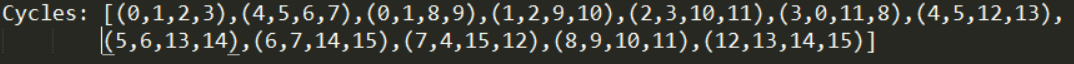
\includegraphics[width=\textwidth]{2d-3d-8} \\ \\
Here the cycles have been reported using vertices, but there is nothing to stop us from keeping connecting pointers between edges and cycles as well. \\ \\
Now we run the two cleaning step (the order is important).\\ \\
In our example, it is easy to see that (4,5,6,7) is completely covered by (0,1,2,3), while (12,13,14,15) is completely covered by (8,9,10,11).  These two pairs are merged, giving: \\ \\
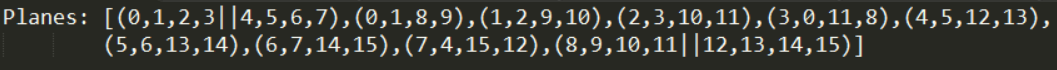
\includegraphics[width=\textwidth]{2d-3d-9} \\ \\

This step can easily be performed in time quadratic on the number of cycles, but better algorithms may exist.\\ \\
The second cleansing step does not affect our example, but would basically involve removing of any planes which are bounded by edges all of which have “degree” three or more. This can be performed in time linear in the number of edges.\\ \\
This kind of an input, though easy to invert, is hardly ever available from a user. The closest one can get then, is when all vertices of the drawing are labeled. Even then, more often than not, there can be a discrepancy w.r.t. which edges exist and which do not.\\ \\

\begin{center}
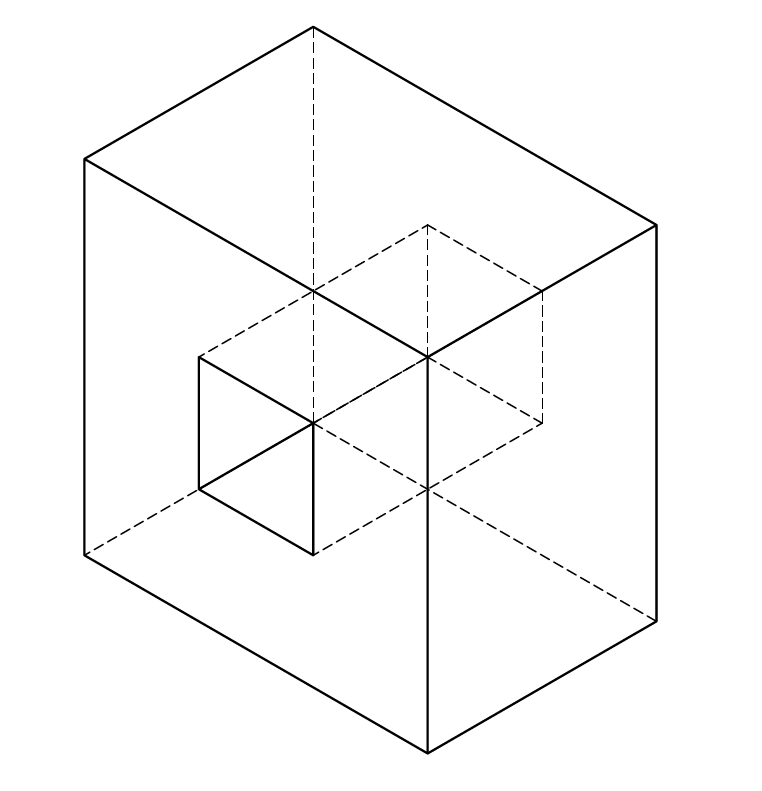
\includegraphics[width = 200pt]{iso} \\
\emph{Isometric view of the exemplar object}
\end{center}
Hereafter, we try to build a more generic approach which would work for unlabeled drawings.

\subsection{Generalized algorithm}
Since Projection drops a dimension, reverting from 2D to 3D is always a complex process. Almost any orthographic projection provides us two views, but this is clearly neither necessary nor sufficient.\\ \\
It is not necessary because it is possible to have pairs of a top view and a front view which can never represent an object. One of the simplest examples is a pair of lines, both parallel to the reference line but having different lines. In this view, we may say that is the projections of both the views onto the reference plane is not identical, then there exists no object satisfying the drawing. This is still not sufficient however Ex: the figure shown probably is not realizable.\\ \\
\begin{center}
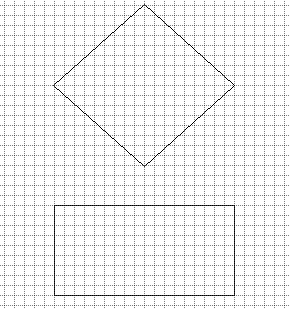
\includegraphics{2d-3d-4}
\end{center}
In general, any edge vertex must have a degree of at least three. If any vertex has an out degree of only two in any view, it must be also present in the other view. In the adjacent drawing, this is clearly not the case. \\ \\
With all these limitations, two views are still not sufficient. Shown here is a set of top and frond views with two possible side views.\\
\begin{center}
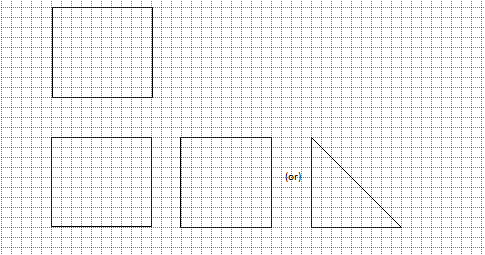
\includegraphics{2d-3d-5}
\end{center}
Given three views, the 3D structure is completely defined, but it also creates the possibility of several types of discrepancies including, but not limited to, the ones discussed for the 2D case.\\ \\
Then what is to be done? Well, we would just rely on what is provided to us and hope for the best. The bare algorithm we shall start with is roughly described as the following:
\begin{itemize}
\item Check that all discovered constraints are satisfied. If not, throw Exception. Note that discovering of constraints is an ongoing process.
\item Project any points present is Top view and not in front view to all lines on the same common coordinate, if doing so does not violate constraints.
\item Repeat above with role of views exchanged.
\item If side view is available apply above procedure to all other pairs of views.
\item Create the points space as a cross product of coordinate sets. Create all edges that are present on atleast one view.
\item Creation of faces is more difficult, but in general, Solid edges need to be covered before dashed ones. 
\item Apply any discovered sanity checks.
\item Show the drawing to the user to suggest any changes.
\end{itemize}
Our primary aim in the rest of the design would be to eliminate the importance of the last step as much as possible. \\ \\
As a final note, the overall process requires us to match sets of points in three drawings, so it definitely reminds one of 3D matching. While 3D matching is surely a much more involved process, it is also proven NP Hard.  All we can hope then is, that we never meet it again.

\section{Minimum number of views for reconstruction}
\emph{Note: This section is developed from the theory of Reference number: 1}
Now, we will discuss the theoretical minimum number of views required for the reconstruction of 3D conics. This number is important as it limits the possibility of exactly reconstructing an object with quadratic surfaces in theory.\\ \\
We first define non-degenerate parallel projection which is useful for subsequent discussions. \\ \\
\emph{Definition1: }\\
Under a parallel projection, if the plane containing the space conic is not perpendicular to the projection plane, then the parallel projection is non-degenerate.  \\ \\
Under the non-degenerate parallel projections, all conics are equivalent, i.e. conics are mapped to conics. It follows, that ellipses, parabolas, and hyperbolas in the drawings are projections of ellipses, parabolas, and hyperbolas respectively. Therefore, if one of the plane curve is conic then the curve in 3D is also conic. \\ \\
Suppose a space conic lies on a plane P and that an object coordinate system $C_P$ is defined such that its $X_P$ and $Y_P$ lie on the plane P. Let C be a global coordinate system in space. Then the global representation $\textbf{x} = [x\,\,\,\,y\,\,\, z\,\,\,\,1]^T$ in C of a global point $\textbf{$x_P$} = [x_p\,\,y_p\,\,z_p\,\,1]^T$ in $C_P$ can be derived by applying transformation of the form:
\begin{align*} \textbf{$x\,\,=\,\,Rx_p + t$} \tag{2.5.1} \end{align*}
where \textbf{R} and \textbf{t} are rotation and translation matrices respectively as discussed before.\\ \\
Thus,\\
\begin{align*} \textbf{X} = 
\begin{bmatrix}
x \\ y \\ z \\ 1 \\ 
\end{bmatrix}
 = 
\begin{bmatrix}
r_{00} & r_{01} & t_0 \\
r_{10} & r_{11} & t_1 \\
r_{20} & r_{21} & t_2 \\
0 & 0 & 0 & 1
\end{bmatrix}
\begin{bmatrix}
x_P \\ y_P \\ 1
\end{bmatrix}
= \textbf{$P \, u_P$}
\tag{2.5.2} \end{align*} 


We now consider the relationship between  space conic and its orthographic projections onto some projection planes. Let \textbf{$c_i$} (i = 1,2,3, ...q) denote the 2D local coordinate system associated with the $i^{th}$ projection plane, and \textbf{$u_i$} = $[x_i, y_i, 1]^T$ denote the homogeneous coordinates of an arbitrary point in its local coordinate system. If \textbf{$C_i$} is a 3X4 matrix whose three columns form an orthogonal basis for this projection subspace, then the transformation from a point \textbf{x} in 3D space to point \textbf{$u_i$} in the projection plane is given by the relation:
\begin{align*} \textbf{$u_i\,\,=\,\,C_i\,x_i$} \tag{2.5.3} \end{align*}

Now we will discuss some theorems that would be useful for our further discussions.\\ \\

\textbf{Theorem: } If a vertex is projected onto three views, its image should be intersection point of two or more non-collinear line segments in at least on view. \\ \\
\textbf{Proof: }The proof is derived by contradiction and the fact that all 2D vertices are intersection points of two or more non-collinear line segments. Suppose that all images of a vertex $v\in V$ in the three views are intersection points (denoted by $P_1, P_2, P_3$) of only two collinear line segments. A vertex can be projected as an intersection point of two collinear line segments only if a face \emph{f} containing that vertex is perpendicular to the projection plane. To satisfy the assumption, all adjacent faces which share that vertex must be perpendicular to the three face planes simultaneously. However a face of an object cannot be perpendicular to all three projection planes simultaneously. Thus contradiction. Hence proved.  $\blacksquare$
\\ \\

\textbf{Theorem: } A tangency edge is projected as a tangency vertex in only one view. \\ \\
\textbf{Proof: }Let$f_1$ and $f_2$ be two curved faces tangent to each other. These faces are projected as two arcs $s_1$ and $s_2$ and they are also tangent to each other since both faces are parallel to the same principal axis. A 2D vertex which is an intersection point of two arcs tangent to each other has tangency type $f_1$ and $f_2$ are projected as two polygons in the other two views. Since two curved faces have $C^1$ continuity, no edges nor vertices would be present in their intersection. Hence proved.  $\blacksquare$
\\ \\

\textbf{Theorem: } Three distinct orthographic projections are sufficient to uniquely recover a space conic. \\ \\
\textbf{Proof: } First of all, suppose that none of the three projections is degenerate. The degenerate case will be considered later. \\Let \textbf{A} be a space conic that lies on a plane P.
\begin{align*} \textbf{$i_P^T\,A\,u_P$} = 0 \tag{2.5.4} \end{align*}
and its projection curves $A_i$ are represented by,
\begin{align*} \textbf{$u_i\,A_i\,u_i$} = 0, \,\,\,\,\,\, i = 1,2,...q \tag{2.5.5} \end{align*}
Substituting the linear transformation of the form $u_i = G_i \, u_P$ into equation 2.5.5, we obtain
\begin{align*} u_P^T\,G_i^T\,A_i\,G_i\,u_P = 0 \tag{2.5.6} \end{align*}
From eqns. 2.5.4 and 2.5.6 we get,
\begin{align*} G_i^T\,A_i\,G_i \, = \, P^T\,C_i^t\,A_i\,C_i\,P \, = \, A, \,\,\,\,\, i=1,2,...q \tag{2.5.7} \end{align*}
where \textbf{A} and \textbf{P} are known matrices. By Bernstein special theorem [2], we can derive that the system of polynomial equations in eqn. 2.5.7 is solvable. Hence sufficient. \\ \\
Further, consider the special case where at least one of the orthographic projections is degenerate. If so, then the projection of conic onto this plane is a straight line. By definition of orthographic projections, we can determine the plane on which the conic lies, which is obtained by extending the straight line along the degenerate projection direction. Since at least one of the projections of the conic is also a conic, we locate the center point of the space conic by finding its corresponding points in the other two views. Accordingly the matrix \textbf{P} is obtained. To reconstruct the space conic we solve $P^T\,C_f^T\,A_f\,C_f\,P = A$ for A, where subscript f indicates front view. In this case also sufficient. Hence proved.  $\blacksquare$
\\ \\
\emph{Other such theorems can be seen in reference 8.}

\chapter{Mathematical Model : OpenGL}
\section{Introduction}
We implement perspective projection using a perspective transformation. Here we describe the perspective transformation used by OpenGL; DirectX uses a slightly different version, we mention that. \\ \\
In its raw form, perspective transformation involves division; it is decidedly neither linear, see Chapter 1, and looks rather ugly, and so might not be expected to be implementable by our beloved matrices. However, owing again to the marvel of homogeneous coordinates, we are able to make it implementable by a matrix. \\ \\
The essence of perspective projection is shown in Figure 3.1; a line PQ in the 3D world is projected onto P’Q’ on the projection plane. C is the centre of projection. In orthographic (parallel) projection, Figure 8.4(b) the rays PP’ and QQ’ are parallel to one another and to the line of sight; being parallel they do not meet at a point. \\ \\
\emph{Note: in cameras and in eyes, the projection plane is behind the centre of projection. In our virtual camera in OpenGL or DirectX we can place the camera in front of the centre of projection; there is no difference in the effect — except that now image objects do not appear upside down.}
\\ \\
\begin{center}
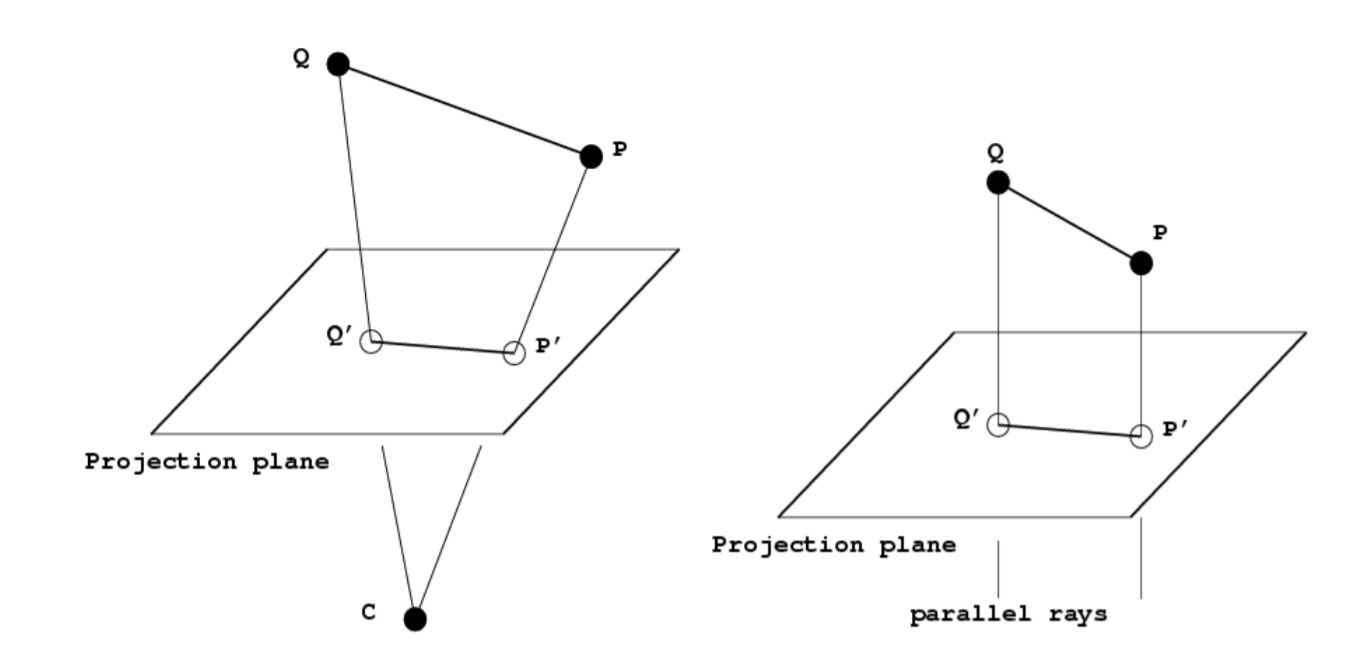
\includegraphics[width=\textwidth]{3-1}
\\ Figure 3.1: Projections: a
\end{center}

\section{Geometry of Perspective}
Figure 3.2 shows a horizontal cross-section of geometry of perspective projection; the vertical cross-section would look similar and would show the x-axis in place of the y-axis. The z-axis is pointing in the negative direction — in OpenGL the centre of projection is always at the origin and
pointing along the negative z-axis. \\ \\
The projective plane is at a distance e in front of the centre of projection. A point $P = (p_x , p_y , p_z )$ is projected onto $(x, y,-e)$.
\\ \\
\begin{center}
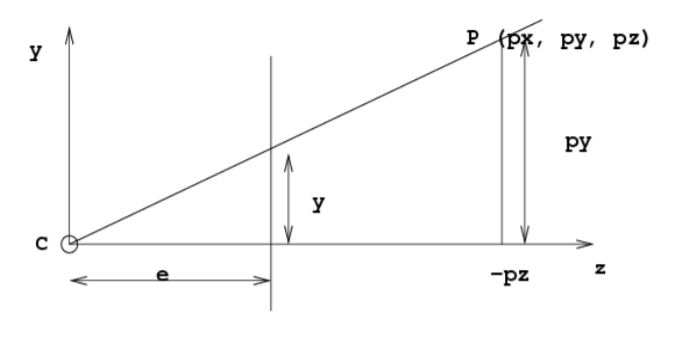
\includegraphics[width=300pt]{3-2}
\\ Figure 3.2: Perspective projection, cross-section
\end{center}
By similar triangles, we have:
\begin{align*} y = -e p_y/p_z \tag{3.1} \end{align*}
If we imagine a similar diagram for x, we have:
\begin{align*} x = -e p_x/p_z \tag{3.2} \end{align*}
Also, 
\begin{align*} z = -e \tag{3.3} \end{align*}
that is all z values get reduced to -e, rather like the simple orthographic projections in chapter 2 where projection onto the x-axis simply reduces the y value to 0 and projection onto the y-axis reduces the x value to 0. Later, we’ll see that OpenGL does not squash z coordinates to one value, and that it transforms them into a set of values that are useful for determining hidden surfaces during rendering. 

\section{OpenGL glFrustum}
The chief method of defining a perspective projection in OpenGL is to define a frustum of a pyramid using glFrustum, see Figure 3.3.
\\ \\
\begin{center}
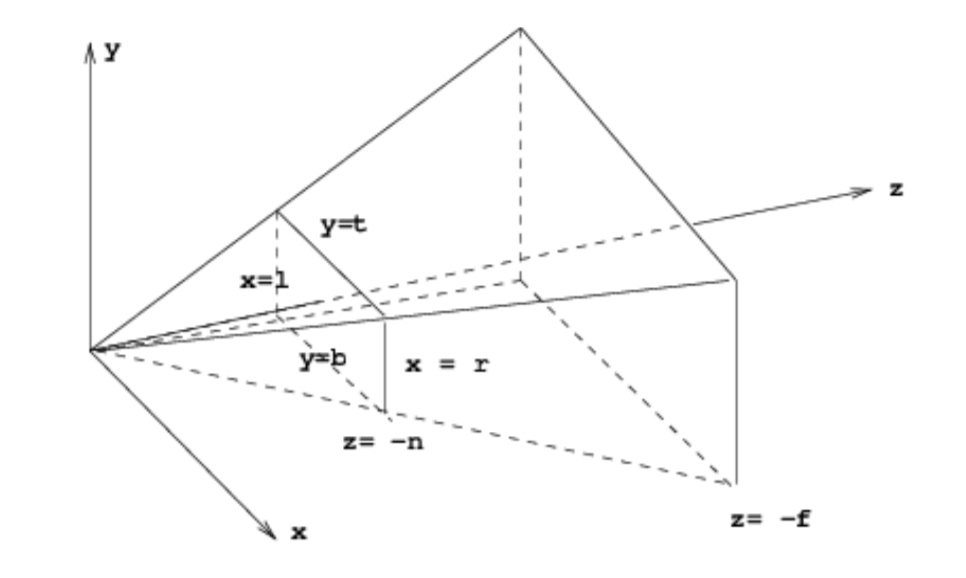
\includegraphics[width=300pt]{3-3}
\\ Figure 3.3: Perspective view frustum volume defined by glFrustum
\end{center}
glFrustum takes six arguments:\\ \\
$ void \, dlFrustum(GLdouble lefrt, GLdouble right, GLdouble bottom, GLdouble top,\\ GLdouble near, GLdouble far). $ \\ \\
Respectively, these the left and right (x-axis), and the bottom and top (y-axis) extents of the field of view; -near is the z position of the projection plane. In addition, rendering is limited to the frustum defined by left, right, bottom, top, near, far; anything outside is not rendered and these
form a 3D clipping region. In Figure 3.3 these are abbreviated l, r, b, t, n, f . \\ \\
OpenGL maps the frustum given by l, r, b, t, n, f to the homogeneous clip space cube shown in Figure 3.4. It maps: $l \mapsto -1, r \mapsto +1, b \mapsto -1, t \mapsto +1$. \\ \\
Also, to use in hidden surface removal, it retains mapped z coordinates; it maps z coordinates thus: $n 7\mapsto -1, f \mapsto +1$; notice that this reverses the direction of the z axis.
\\ \\
\begin{center}
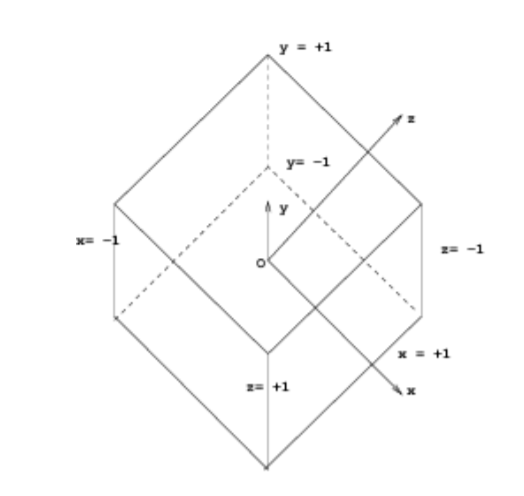
\includegraphics[width=200pt]{3-4}
\\ Figure 3.4 : Homogeneous clip space cube
\end{center}

\section{Derivation of Perspective Transformations}
In Figure 3.3 the e of the Figure 3.2 becomes n; consequently the simple raw projection eqns 3.1 and 3.2 become
\begin{align*} y = -n p_y/p_z \tag{3.4} \end{align*}
For x, we likewise have
\begin{align*} x = -n p_x/p_z \tag{3.5} \end{align*}
Now, as noted in the previous subsection, OpenGL maps $x = l \mapsto x' = -1, x = r \mapsto x'= +1 and y = b \mapsto y' = -1, y = t \mapsto y' = +1$, see Figure 3.4. We can use a handy formula, namely eqn. 3.6,
\begin{align*} v = (u - u_0) \frac{v_1 - v_0}{u_1 - u_0} + v_0 \tag{3.6} \end{align*}
which maps $ u_0 \mapsto v_0 and u_1 \mapsto v_1 $, i.e. in the present case $ x = l \mapsto x'= -1 and x = r \mapsto x'= +1$ and likewise for y, y'. \\ \\
For the x mapping, eqn 3.6 gives:
\begin{align*} x'&= (x-l)\frac{1-(-1)}{r-l} - 1, \tag{3.7} \\
&= (x-l)\frac{2}{r-l} -1,\\
&= \frac{2(x-l)-r+l}{r-l},\\
&= \frac{2x-2l-r+l}{r-l}
\end{align*}
So,
\begin{align*} x'= \frac{2x - (r+l)}{r-l} \tag{3.8} \end{align*}
Substituting eqn 3.5 into 3.8 gives,
\begin{align*} x'= \frac{2n \frac{-p_x}{p_z}- (r+l)}{r-l} \tag{3.9} \end{align*}
and there is a similar equation for y',
\begin{align*} y'= \frac{2n \frac{-p_y}{p_z}- (t+b)}{t-b} \tag{3.10} \end{align*}
Thinking ahead to the required form, eqns 3.9 and 3.10 can be rewritten
\begin{align*} -x'p_z = \frac{2np_x + (r+l)p_z}{r-l} \tag{3.11} \end{align*}
and,
\begin{align*} -y'p_z= \frac{2np_y+(t+b)p_z}{t-b} \tag{3.12} \end{align*}
Now $p_z$  has to be mapped; the problem here is that the rasterisation stage needs the reciprocal of $p_z (\frac{1}{p_z})$ rather than $p_z$ so that we need $z'= a(\frac{1}{p_z}) + b$. Eqn 3.6 is still usable if we define $s = \frac{1}{p_z}$ and define the mapping $s = -\frac{1}{n} \mapsto z'= -1 and s  = -\frac{1}{f} \mapsto z'= +1$, so eqn 3.6 gives,
\begin{align*} z'&= \frac{(\frac{1}{p_z}+ \frac{1}{n})(1+1)}{(-\frac{1}{f} + \frac{1}{n})} - 1, \tag{3.13} \\
&= \frac{2\frac{fn}{p_z} +2f}{-n+f} -1,\\
&= \frac{2fn\frac{-1}{p_z} +2f}{f-n} ,\\
-z'p_z &= \frac{-2fn -2fp_z +p_zf -p_zn}{f-n} + p_z ,\\
\end{align*}
and finaly,
\begin{align*} -z'p_z &= \frac{-p_z(f+n)-2fn}{f-n} \tag{3.14} \\
\end{align*}
From the projected 3D point $\textbf{p'} = (x', y', z')$ (the mapped image of $(p_x, p_y, p_z)$) we now create the 'homogeneous' coordinates for$\textbf{p'} = (-x'p_z, y'p_z, -z'p_z, -p_z)$; note the $-p_z$ in the w component. Then summarize eqns. 3.11, 3.13 and 3.14 as
\begin{align*}  -x'p_z &= \frac{2np_x}{r-l}p_x + \frac{r+l}{r-l}p_z, \tag{3.15} \\ -y'p_z &= \frac{2n}{t-b}p_y + \frac{t+b}{t-b}p_z, \tag{3.16}
\end{align*}
and
\begin{align*} -z'p_z &= -\frac{f+n}{f-n}p_z - \frac{2nf}{f-n} \tag{3.17} \\
\end{align*}
The whole projective transformation can now be written in terms of a matrix multiplication and homogeneous coordinates,
\begin{align*} 
\begin{bmatrix}
-x'p_z \\ -y'p_z \\ -z'p_z \\ w' \\ 
\end{bmatrix} = 
\begin{bmatrix}
\frac{2n}{r-l} & 0 & \frac{r+l}{r-l} & 0 \\
0 & \frac{2n}{t-b} & \frac{t+b}{t-b} & 0 \\
0 & 0 & -\frac{f+n}{f-n} & -\frac{-2nf}{f-n} \\
0 & 0 & -1 & 0 \\
\end{bmatrix}
\begin{bmatrix}
p_x \\ p_y \\ p_z \\ 1 \\
\end{bmatrix} \tag{3.18}
\end{align*}
Recall $glFrustum$, where we now use the same symbols as in eqn. 3.18:\\ \\
$void \, glfrustum(GLdouble l, GLdouble r, GLdouble b, GLdouble t, GLdouble n, \\ GLdouble f).$\\ \\
Figure 3.8 shows the final transformation stages in full context.
\\ \\
\begin{center}
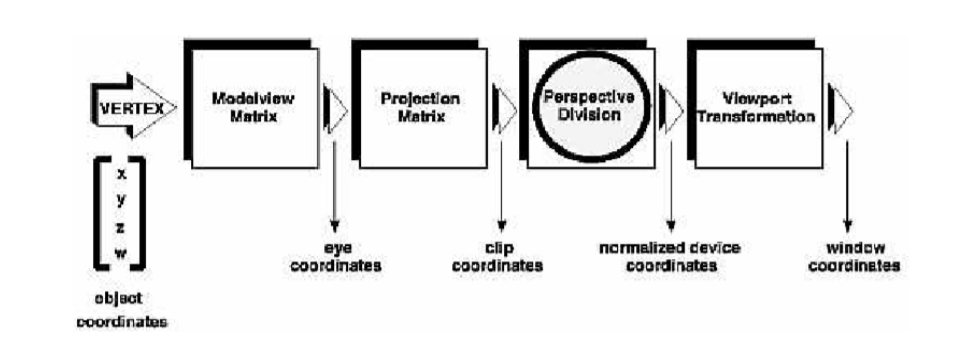
\includegraphics[width=250pt]{3-8}
\\ Figure 3.8: Vertex transformation pipeline. \\
\end{center} 


\section{Orthographic Projection}
In an orthographic or parallel projection, the projection rays are parallel to one another and to the camera viewing direction. In addition lack of perspective distortion means that (in OpenGL) true z coordinates can be interpolated linearly (rather than reciprocal (1/z) values). \\ \\
Consequently all that needs to be done for x and y is a mapping as given by eqn. 3.8 for x,
\begin{align*} x'&= \frac{2x - (r+l)}{r-l}, \tag{3.19} \\
&= \frac{2x}{r-l} - \frac{r+l}{r-l}, \tag{3.20} \\
\end{align*}
and the same for y,
\begin{align*} y'&= \frac{2x}{t-b} - \frac{t+b}{t-b}, \tag{3.21} \\
\end{align*}
The z coordinate mapping is $-f \mapsto -1, -n \mapsto +1$, so,
\begin{align*} z'&= \frac{-2z}{f-n} - \frac{f+n}{f-n}, \tag{3.22} \\
\end{align*}
We note that eqns. 3.20, 3.21 and 3.22 represent an affine transformation, i.e. scale plus translate. Their matrix representation is given by eqn. 3.23; this is the projection matrix generated by OpenGL function glOrtho:\\ \\
$ void \, glOrtho(GLdouble left, GLdouble right, \\ GLdouble bottom, GLdouble top, GLdouble near, GLdouble far)$.\\ \\
\begin{align*} 
\begin{bmatrix}
-x' \\ -y' \\ -z' \\ w' \\ 
\end{bmatrix} = 
\begin{bmatrix}
\frac{2}{r-l} & 0 & 0 & -\frac{r+l}{r-l} \\
0 & \frac{2}{t-b} & 0 & -\frac{t+b}{t-b}  \\
0 & 0 & -\frac{-2}{f-n} & -\frac{f+n}{f-n}  \\
0 & 0 & 0 & 1 \\
\end{bmatrix}
\begin{bmatrix}
p_x \\ p_y \\ p_z \\ 1 \\
\end{bmatrix} \tag{3.23}
\end{align*}
Now these transformation matrices are used with the algorithm discussed in Chapter 2 to find the correct orthographic projections of the 3D model. 

\section{Reconstruction: 3D back from 2D}
We now discuss the phase of reconstruction, i.e. using 2D orthographic projections to develop the corresponding 3D model and build on the ideas discussed in chapter 2 to formulate an implementable algorithm suitable for unlabeled vertices and unlabeled edges.\\ \\
 For convenience, probable 3D vertices, probable 3D edges, probable faces, probable 3D sub-objects are written as \emph{p-vertices, p-edges, pfaces,
p-subobjects}, respectively. 
\subsection{Step 1 : 2D vertices and 2D lines}
In this step we process the input data and remove certain redundancies. All the points and lines that are input by the user are 2D vertices and 2D lines. First, all the duplicate specifications of these vertices, if any,
are removed. Next. since the user is not required to input the intersection points of two straight lines, it is determined if an intersection point exists and if it does, it is added to the list of vertices. Finally, the collinear lines of the same type, namely, solid or dashed, are combined to form one line. \\ \\
The intersection of two lines is determined using the following algorithm. Let the two lines under consideration be KL and MN. The parametric equations
for these lines can be written as: 
\begin{align*}
x = x_K + (x_L - x_K)s \\
y = y_K + (y_L - y_K)s \tag{3.24}
\end{align*}
for line KL and
\begin{align*}
x = x_M + (x_N - x_M)t \\
y = y_M + (y_N - y_M)t \tag{3.25}
\end{align*}
for line MN, where s and t are the parameters. The point of intersection, J, satisfies both Eqns. (3.24) and (3.25). One can obtain the values of the  parameters s and t at J as: 
\begin{align*}
s_J = \frac{(x_N-x_M)(y_M-y_K)-(y_N-y_M)(x_M-x_K)}{(x_N-x_M)(y_L-y_K)-(y_N-y_M)(x_L-x_K)} \tag{3.26} \\
t_J = \frac{(x_L-x_K)(y_M-y_K)-(y_L-y_K)(x_M-x_K)}{(x_N-x_M)(y_L-y_K)-(y_N-y_M)(x_L-x_K)} \tag{3.27}
\end{align*}
If both $s_J$ and $t_J$ are in the range of 0 to 1, then the intersection occurs within the two line segments and is given by 
\begin{align*}
x_J = x_k + (x_L-x_K)s_J = x_M + (x_N - x_M)t_j \\
y_J = y_K + (y_L-y_K)s_j = y_m + (y_N - y_M)t_J \tag{3.28}
\end{align*}
This point is then added as a 2D vertex. If $s_J < 0$ or $s_J>1$ or $t_J<0$ or $t_J>1$, then the line segments intersect outside their span and intersection not valid.

\subsection{Step 2 : Probable 3D vertices}
A list of probable 3D vertices is constructed in this step. If any two 2D vertices, belonging to different views, have the same coordinate .value for the shared coordinate axis, then the third view is searched for the 2D vertex which has the same values as the remaining two coordinates from the original two 2D vertices under consideration. If the search is successful then a 3D p-vertex containing the common x, y, z coordinates from three 2D vertices is found. This procedure is carried out for all the 2D vertices.

\subsection{Step 3 : Probable 3D edges }
Recursive in nature, this step involves both the generation of p-edges and checking the validity of p-vertices. If any p-vertex is found to be invalid, that p-vertex is deleted and the procedure goes back to the beginning of this step. \\ \\
A straight line which connects any two p-vertices is a p-edge provided the
projections of this 3D edge can be found in all the three input views. Since this algorithm deals with planar objects, these projections can appear as 2D lines or as a 2D vertex. Whenever this test is satisfied the p-edge formed under consideration is compared with the previously generated p-edges. If the most recently generated p-edge contains any one of the previously generated p-edges, then the most recently generated p-edge is not included in the p-edges table. On the other hand, if any of the previously generated p-edges contain the most recently generated p-edge then all those previously
generated p-edges are deleted. The criterion behind this test is not to store overlapping p-edges. \\ \\
The p-edges are stored in terms of their end points. From this, a table that
gives the p-edge numbers to which each p-vertex belongs is created. Since the algorithm deals with solid objects, each p-vertex should belong to at least three p-edges. Ira p-vertex belongs to less than three p-edges, then it is assumed to be a false p-vertex and is deleted. Whenever a p-vertex is deleted, the validity of the p-edges is no longer guaranteed; hence the process returns to the beginning of this step (i.e.. step 3). If none of
the p-vertices is deleted then the process advances to the next step. 

\subsection{Step 4 : Probable faces}
In this step, a list of probable planar faces is constructed.
This step is composed of the following sub-steps:
\begin{enumerate}
\item Determination of planar surfaces
\item Generation of p-edge closed loops
\item P-edge loop relationships
\item Formation of p-faces
\item Testing of 2D dashed lines
\end{enumerate}
\emph{Determination of planar surfaces:}\\
 The list of p-edges is searched to find out a pair of p-edges with a common p-vertex. A planar surface passing through these p-edges can be represented mathematically as: 
\begin{align*}
 ax+by+cz+d=0
\end{align*}
Given KJ and JL as the p-edges with $(x_J, y_J, z_J), (x_K, y_K, z_K) and (x_L, y_L, z_L)$ as the coordinates of the p-vertices J, K and L, respectively, the equation of the plane through these points is given as 
\begin{align*}
\begin{bmatrix}
x-x_J & y-y_J & z-z_J \\
x_K-x_J & y_K-y_J & z_K-z_J \\
x_L-x_J & y_L-y_J & z_L-z_J \\
\end{bmatrix} = 0
\end{align*}
Then, coefficients a,b,c,d can be determined.

\subsection{Step 5 : Generation of 3D Object}
In this step the p-faces are connected to form p-sub-objects which are then classified as certain and uncertain p-sub-objects. To connect p-faces, the cross-product and dot product between the surface normals are used. \\ \\
Any p-face is chosen as the starting p-face, With this p-face as the  reference p-face, the connecting p-faces are found by making use of Table 1. Next, with any one of the just found p-faces as the reference p-face. its connecting p-faces are found. This procedure continues until all the connecting p-faces are found. At
this stage, a p-sub-object is said to have been found. In order to find the next p-sub-object, any p-face that has not been used so far is chosen as the reference p-face and the procedure repeated. When both sides of all the p-faces have been used, the search for all the p-sub-objects is finished. While forming a p-sub-object, if both sides of a p-face are required, then that p-face is assumed to be a false one and is deleted: the process in that case goes back to the beginning of step 5. 
\begin{center}
\begin{tabular}{ |p{2cm}|p{3cm}|p{3cm}|p{2cm}|p{2cm}| } 
\hline
Reference p-face & Direction of vector crossproduct w.r.t reference p-edge & Direction of traversal of shared p-edge & face connecting angle & Side to be chosen \\ \hline \hline
o & opposite & same & 360-$\theta$ & s \\ 
o & opposite & opposite & 180-$\theta$ & o \\ 
o & same & same & $\theta$ & s \\ 
o & same & opposite & 180+$\theta$ & o \\ 
s & opposite & same & $\theta$ & o \\ 
s & opposite & opposite & 180+$\theta$ & s \\ 
s & same & same & 360-$\theta$ & o \\ 
s & same & opposite & 180-$\theta$ & s \\
\hline
\end{tabular}
\end{center}
Note: o means the face that bounds the opposite side of the surface normal, s means the face that bounds the same side of the surface normal. \\ \\
After getting all the 2D lines, collinear 2D lines which are of the same type are joined together and stored as a single 2D line. The regenerated 2D lines
are compared with the original 2D lines; if they match exactly, then the assembled p-object is one of the solutions or the only solution.\\ \\
This set of vertices and edges may contain several \textbf{ghosts} (non existing vertices, edges or faces), these can be removed using heuristic approach to find the minimum number of vertices and edges required to match the given projections. To start off,\textbf{ we first consider the reconstruction problem with labeled vertices and unlabeled edges} which is the case mostly, and then tackle the general problem of unlabeled vertices and unlabeled edges later. An example explaining this approach only for the case of edge reduction is discussed next, where labeled vertices and unlabeled edges are used for reconstruction. This algorithm can be extended for face reduction as well. 

\section{Exemplar problem for 2D to 3D reconstruction}
Since real drawings never contain labeled edges, we here try to use a simplified heuristic implementation of algorithm to illustrate how to recover the edges of the wireframe, given all the points and projected edges and remove redundant vertices and edges that came up by the last algorithm discussed. This can be further extended for faces and computation can be done to determine full model. The Algorithm takes as input:\\
\begin{center}
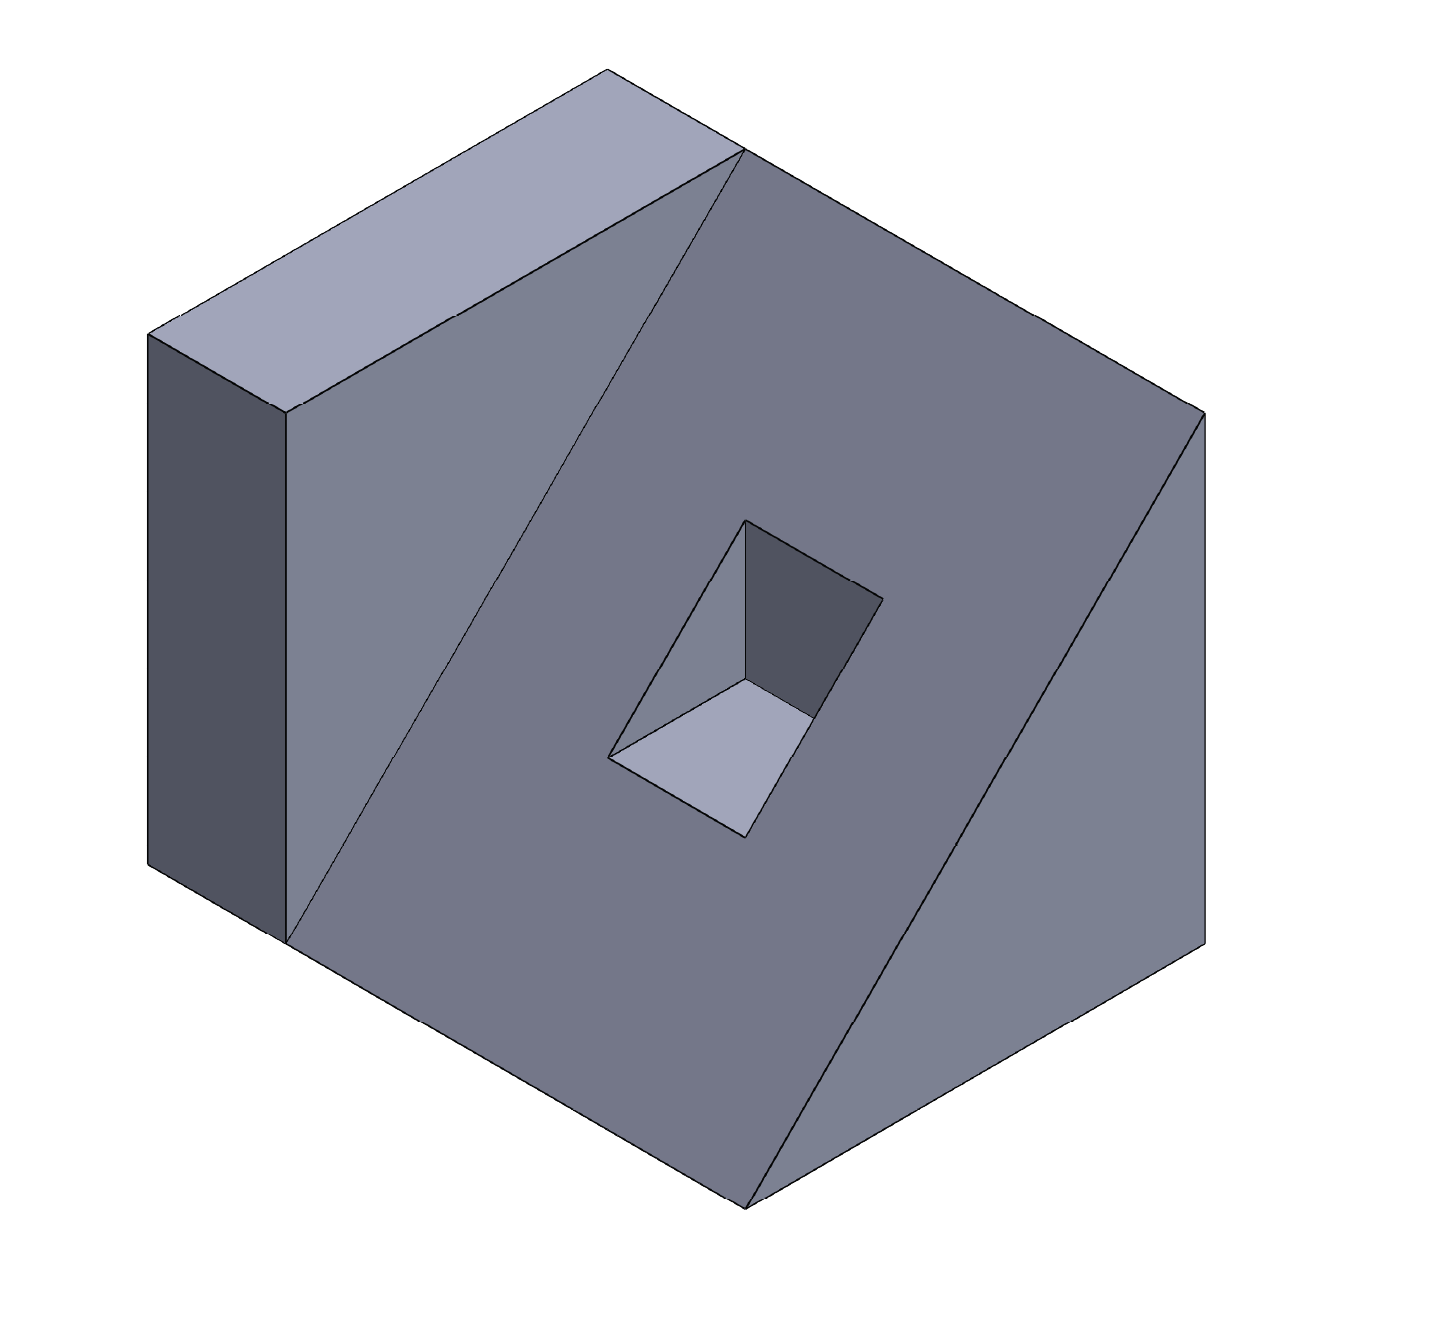
\includegraphics[width = 200pt]{solid2} \\
\emph{Solid object used for this example}
\end{center}
\begin{itemize}
\item Projected vertices and which real vertices they correspond to. Real vertices are named using some symbols, and this name is identical in all projections.
\item Edges between projected vertices. As a convention, if a projected edge passes over multiple vertices, it is written as a set of smaller edges between two vertices.
\end{itemize}
Given these, our algorithm proceeds in following steps:
\begin{enumerate}
\item True vertex set is extracted. This is possible using the procedure already described, using labels instead of projections. 
\item The adjacency matrix is initialized for the complete graph.
\item Iterate over each view:
\begin{enumerate}
\item Add missing edges, i.e. edges that can be formed by adding to collinear connected edges
\item Remove all edges whose projection does not exist on this view from the adjacency matrix
\end{enumerate}
\item Complete graph by heuristics, if required
\begin{enumerate}
\item Each edge must get at least 3 non-coplanar edges
\item Three edges from a vertex are coplanar iff two of them are collinear
\item Two edges should not intersect except at vertices.
\item No vertex may lie on an edge other than its end points
\end{enumerate}
\end{enumerate}
\begin{itemize}
\item No vertex may lie on an edge other than its end points
\item The edge is completely covered by another edge
\end{itemize}
The first of these is guaranteed to be overcome with even two views: two points can be same in at most two coordinates. The second one is a bit harder, eg 3 edges of a cube are not visible even after looking at 3 views. Therefore, some heuristics may be needed. Note that while this does not guarantee a solution, is does so almost always.
Consider the following example: \\
\begin{figure}[H]
\begin{subfigure}{0.5\textwidth}
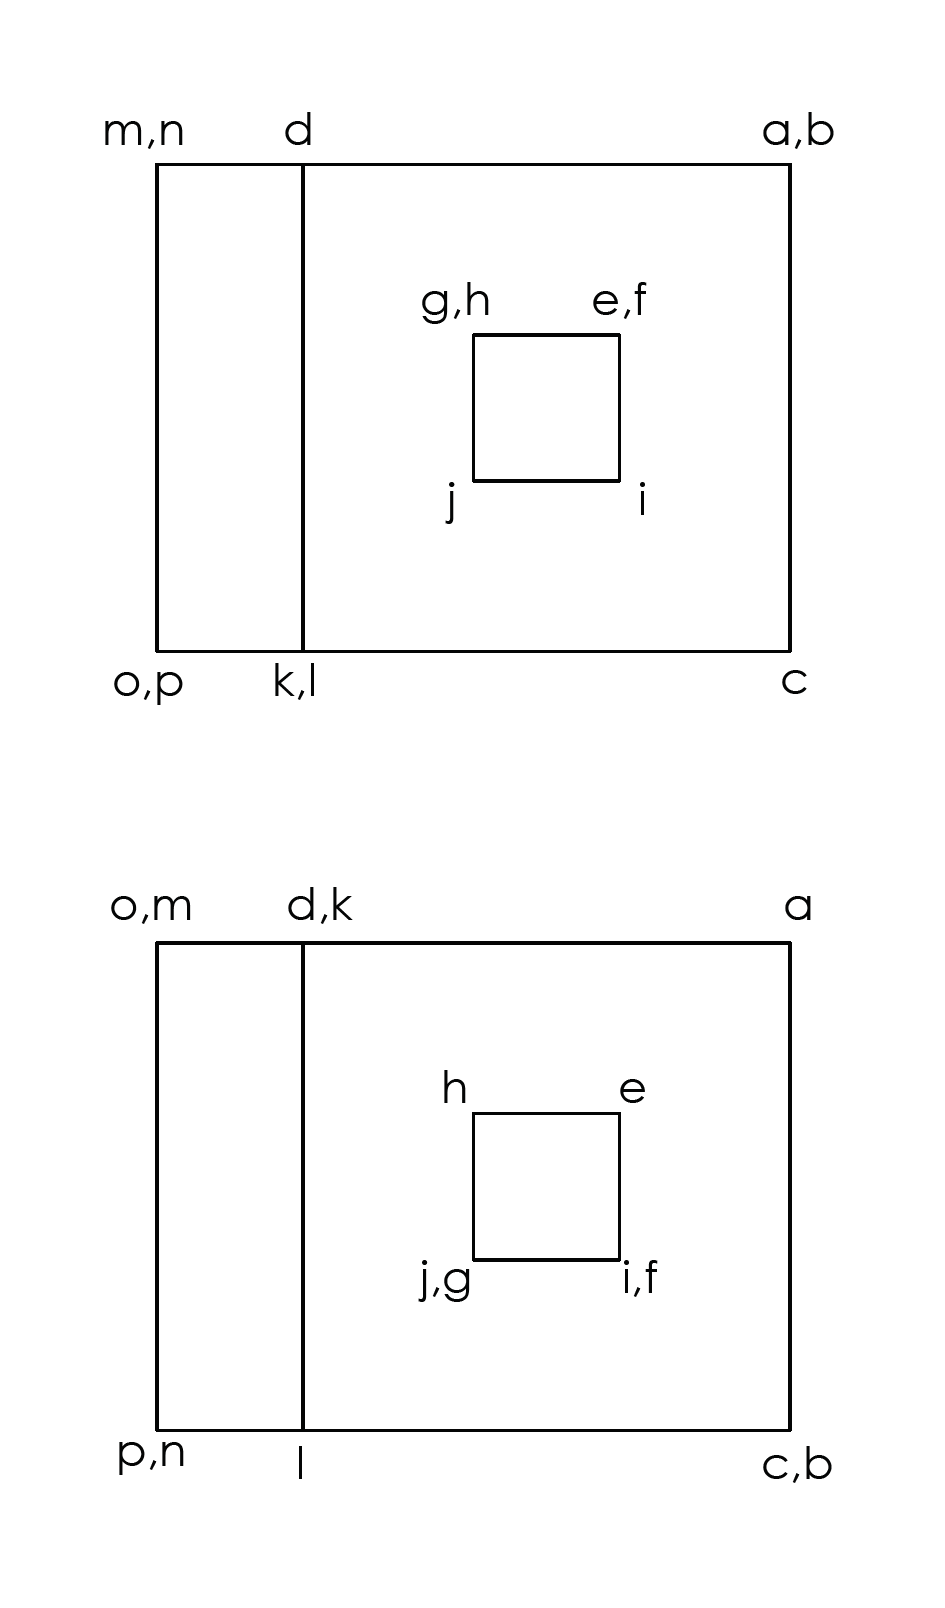
\includegraphics[width = 170pt]{ortho2} \\
\caption{Orthographic projection of the example}
\end{subfigure}
\begin{subfigure}{0.5\textwidth}
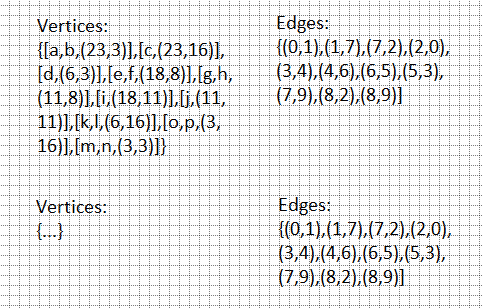
\includegraphics[width = 200pt]{vande1} \\
\caption{Vertices and edges in top and front views}
\end{subfigure}
\end{figure}
Note that the naming does not follow some of the conventions.\\
The first step is skipped as it is rather easy.\\ \\
We start off with the adjacency matrix: (to show the power of this approach, let us assume that excessive edges have been declared probable and in the extreme case - all)\\ \\
\begin{center}
\begin{tabular}[width = \textwidth]{ |c|c|c|c|c|c|c|c|c|c|c|c|c|c|c|c|c| } 
\hline
  & a & b & c & d & e & f & g & h & i & j & k & l & m & n & o & p \\ \hline \hline
a &   &   &   &   &   &   &   &   &   &   &   &   &   &   &   &   \\ \hline
b & 1 &   &   &   &   &   &   &   &   &   &   &   &   &   &   &   \\ \hline
c & 1 & 1 &   &   &   &   &   &   &   &   &   &   &   &   &   &   \\ \hline
d & 1 & 1 & 1 &   &   &   &   &   &   &   &   &   &   &   &   &   \\ \hline
e & 1 & 1 & 1 & 1 &   &   &   &   &   &   &   &   &   &   &   &   \\ \hline
f & 1 & 1 & 1 & 1 & 1 &   &   &   &   &   &   &   &   &   &   &   \\ \hline
g & 1 & 1 & 1 & 1 & 1 & 1 &   &   &   &   &   &   &   &   &   &   \\ \hline
h & 1 & 1 & 1 & 1 & 1 & 1 & 1 &   &   &   &   &   &   &   &   &   \\ \hline 
i & 1 & 1 & 1 & 1 & 1 & 1 & 1 & 1 &   &   &   &   &   &   &   &   \\ \hline
j & 1 & 1 & 1 & 1 & 1 & 1 & 1 & 1 & 1 &   &   &   &   &   &   &   \\ \hline
k & 1 & 1 & 1 & 1 & 1 & 1 & 1 & 1 & 1 & 1 &   &   &   &   &   &   \\ \hline
l & 1 & 1 & 1 & 1 & 1 & 1 & 1 & 1 & 1 & 1 & 1 &   &   &   &   &   \\ \hline
m & 1 & 1 & 1 & 1 & 1 & 1 & 1 & 1 & 1 & 1 & 1 & 1 &   &   &   &   \\ \hline
n & 1 & 1 & 1 & 1 & 1 & 1 & 1 & 1 & 1 & 1 & 1 & 1 & 1 &   &   &   \\ \hline
o & 1 & 1 & 1 & 1 & 1 & 1 & 1 & 1 & 1 & 1 & 1 & 1 & 1 & 1 &   &   \\ \hline
p & 1 & 1 & 1 & 1 & 1 & 1 & 1 & 1 & 1 & 1 & 1 & 1 & 1 & 1 & 1 &   \\ \hline
\hline
\end{tabular}
\end{center}
\vfill
Now, we look at the top view, and eliminate all edges not present there: \\ \\
\begin{center}
\begin{tabular}[width = \textwidth]{ |c|c|c|c|c|c|c|c|c|c|c|c|c|c|c|c|c| } 
\hline
  & a & b & c & d & e & f & g & h & i & j & k & l & m & n & o & p \\ \hline \hline
a &   &   &   &   &   &   &   &   &   &   &   &   &   &   &   &   \\ \hline
b & 1 &   &   &   &   &   &   &   &   &   &   &   &   &   &   &   \\ \hline
c & 1 & 1 &   &   &   &   &   &   &   &   &   &   &   &   &   &   \\ \hline
d & 1 & 1 &   &   &   &   &   &   &   &   &   &   &   &   &   &   \\ \hline
e &   &   &   &   &   &   &   &   &   &   &   &   &   &   &   &   \\ \hline
f &   &   &   &   & 1 &   &   &   &   &   &   &   &   &   &   &   \\ \hline
g &   &   &   &   & 1 & 1 &   &   &   &   &   &   &   &   &   &   \\ \hline
h &   &   &   &   & 1 & 1 & 1 &   &   &   &   &   &   &   &   &   \\ \hline 
i &   &   &   &   & 1 & 1 &   &   &   &   &   &   &   &   &   &   \\ \hline
j &   &   &   &   &   &   & 1 & 1 & 1 &   &   &   &   &   &   &   \\ \hline
k &   &   & 1 & 1 &   &   &   &   &   &   &   &   &   &   &   &   \\ \hline
l &   &   & 1 & 1 &   &   &   &   &   &   & 1 &   &   &   &   &   \\ \hline
m & 1 & 1 &   & 1 &   &   &   &   &   &   &   &   &   &   &   &   \\ \hline
n & 1 & 1 &   &   &   &   &   &   &   &   &   &   & 1 &   &   &   \\ \hline
o &   &   & 1 &   &   &   &   &   &   &   & 1 & 1 & 1 & 1 &   &   \\ \hline
p &   &   & 1 &   &   &   &   &   &   &   & 1 & 1 & 1 & 1 & 1 &   \\ \hline
\hline
\end{tabular}
\end{center}
\pagebreak
And then the front view:
\begin{center}
\begin{tabular}[width = \textwidth]{ |c|c|c|c|c|c|c|c|c|c|c|c|c|c|c|c|c| } 
\hline
  & a & b & c & d & e & f & g & h & i & j & k & l & m & n & o & p \\ \hline \hline
a &   &   &   &   &   &   &   &   &   &   &   &   &   &   &   &   \\ \hline
b & 1 &   &   &   &   &   &   &   &   &   &   &   &   &   &   &   \\ \hline
c & 1 & 1 &   &   &   &   &   &   &   &   &   &   &   &   &   &   \\ \hline
d & 1 &   &   &   &   &   &   &   &   &   &   &   &   &   &   &   \\ \hline
e &   &   &   &   &   &   &   &   &   &   &   &   &   &   &   &   \\ \hline
f &   &   &   &   & 1 &   &   &   &   &   &   &   &   &   &   &   \\ \hline
g &   &   &   &   &   & 1 &   &   &   &   &   &   &   &   &   &   \\ \hline
h &   &   &   &   & 1 &   & 1 &   &   &   &   &   &   &   &   &   \\ \hline 
i &   &   &   &   & 1 & 1 &   &   &   &   &   &   &   &   &   &   \\ \hline
j &   &   &   &   &   &   & 1 & 1 & 1 &   &   &   &   &   &   &   \\ \hline
k &   &   &   & 1 &   &   &   &   &   &   &   &   &   &   &   &   \\ \hline
l &   &   & 1 & 1 &   &   &   &   &   &   & 1 &   &   &   &   &   \\ \hline
m & 1 &   &   & 1 &   &   &   &   &   &   &   &   &   &   &   &   \\ \hline
n &   & 1 &   &   &   &   &   &   &   &   &   &   & 1 &   &   &   \\ \hline
o &   &   &   &   &   &   &   &   &   &   & 1 &   & 1 & 1 &   &   \\ \hline
p &   &   & 1 &   &   &   &   &   &   &   &   & 1 & 1 & 1 & 1 &   \\ \hline
\hline
\end{tabular}
\end{center}
Now we begin applying heuristics.\\ \\
The second constraint is violated at m as the edges MN, MO and MP cannot all exist. Also, it is violated at N as MN,NO and NP cannot all exist together. Further, MP and no cannot coexist as the intersect. So, exactly one of MN, MO, MP; exactly one of MN, NO, NP and atleast one of MP, NO must be dropped. An exhaustive search can give that the only stable solution is when MP and NO are dropped. Note that this would be unnecessary if an LHS view was provided and simplified somewhat if a RHS view was provided. \\ \\
The fourth constraint is violated by AM and CP. These two are also dropped. At this point all constraints are satisfied and our algorithm stops.\\ \\
\begin{center}
\begin{tabular}[width = \textwidth]{ |c|c|c|c|c|c|c|c|c|c|c|c|c|c|c|c|c| } 
\hline
  & a & b & c & d & e & f & g & h & i & j & k & l & m & n & o & p \\ \hline \hline
a &   &   &   &   &   &   &   &   &   &   &   &   &   &   &   &   \\ \hline
b & 1 &   &   &   &   &   &   &   &   &   &   &   &   &   &   &   \\ \hline
c & 1 & 1 &   &   &   &   &   &   &   &   &   &   &   &   &   &   \\ \hline
d & 1 &   &   &   &   &   &   &   &   &   &   &   &   &   &   &   \\ \hline
e &   &   &   &   &   &   &   &   &   &   &   &   &   &   &   &   \\ \hline
f &   &   &   &   & 1 &   &   &   &   &   &   &   &   &   &   &   \\ \hline
g &   &   &   &   &   & 1 &   &   &   &   &   &   &   &   &   &   \\ \hline
h &   &   &   &   & 1 &   & 1 &   &   &   &   &   &   &   &   &   \\ \hline 
i &   &   &   &   & 1 & 1 &   &   &   &   &   &   &   &   &   &   \\ \hline
j &   &   &   &   &   &   & 1 & 1 & 1 &   &   &   &   &   &   &   \\ \hline
k &   &   &   & 1 &   &   &   &   &   &   &   &   &   &   &   &   \\ \hline
l &   &   & 1 & 1 &   &   &   &   &   &   & 1 &   &   &   &   &   \\ \hline
m &   &   &   & 1 &   &   &   &   &   &   &   &   &   &   &   &   \\ \hline
n &   & 1 &   &   &   &   &   &   &   &   &   &   & 1 &   &   &   \\ \hline
o &   &   &   &   &   &   &   &   &   &   & 1 &   & 1 &   &   &   \\ \hline
p &   &   &   &   &   &   &   &   &   &   &   & 1 &   & 1 & 1 &   \\ \hline
\hline
\end{tabular}
\end{center}
It is easy to see that this is in fact, the correct adjacency matrix.\\ \\ The generated wireframe is shown below. 
\begin{center}
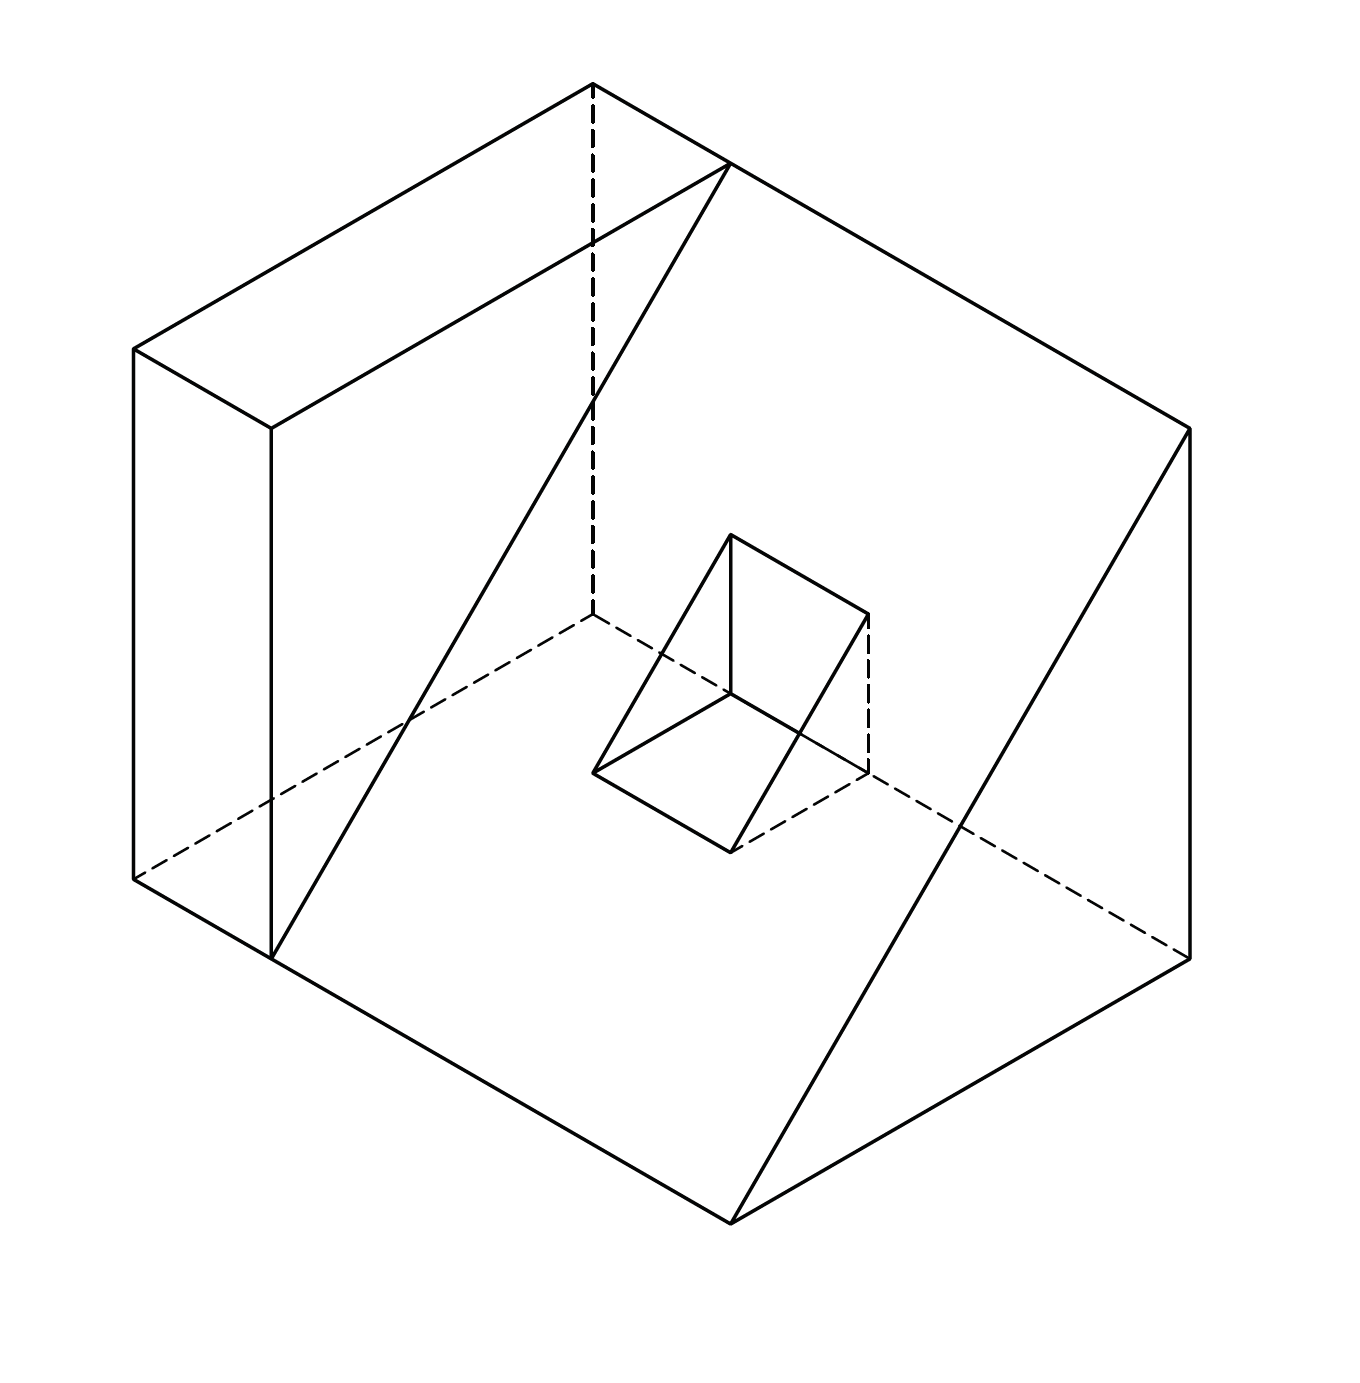
\includegraphics[width = 200pt]{iso2} \\
\emph{Generated 3D model's edges}
\end{center}
As this heuristic approach provides us a correct way to obtain edges of the model, it can be extended to obtain the required faces. This edge limited implementation gives us reasonable confidence to proceed further with our model and implement it to build the required program.
\chapter*{References}
\begin{enumerate}
\item A matrix-based approach to reconstruction of 3D objects from three orthographic views:\\
$http://ieeexplore.ieee.org/document/883948/$
\item DN Berstein, The number of roots of a system of equations, Functional Analysis and its applications, 1975, 9(3), pp. 1-4
\item OpenGL : SuperBible
\item 3D Projections Wikipedia:\\ $https://en.wikipedia.org/wiki/3D_projection$
\item ScratchPixel OpenGL Perspective projections: \\ $https://www.scratchapixel.com/lessons/3d-basic-rendering/perspective-and-orthographic-projection-matrix/building-basic-perspective-projection-matrix$
\item MultiResolution Mathematics of 3D projections:\\
$http://www.multiresolutions.com/strule/jon/www-jgcampbell-com/bscgp1/ \\ grmaths.pdf$
\item Construction of 3D Solid Objects from Orthographic Views: \\
$https://ac.els-cdn.com/0097849389900125/1-s2.0-0097849389900125-main.pdf?_tid=687e87a8-f9d3-11e7-aeef-00000aacb360\& \\acdnat=1516007385_95bbc8703eeef965232455a47c69c334$
\item Fast 3D solid model reconstruction:
$https://ac.els-cdn.com/S0010448597000547/1-s2.0-S0010448597000547-main.pdf?_tid=02520032-f9dc-11e7-a247- \\ 00000aacb362\&acdnat=1516011079_ef49322c2d3a1bc2136796b1399ff1b9$
\end{enumerate}




%----------------------------------------------------------------------------------------
%	BIBLIOGRAPHY
%----------------------------------------------------------------------------------------

\printbibliography[heading=bibintoc]

%----------------------------------------------------------------------------------------

\end{document}  
